\documentclass[11pt,letterpaper]{article}
\usepackage[T1]{fontenc}
\usepackage[utf8]{inputenc}
\usepackage{lmodern}
\usepackage[margin=1in,headheight=15pt]{geometry}
\usepackage{microtype,amsmath,amssymb,amsthm,mathtools}
\usepackage{booktabs,longtable,array,enumitem,graphicx,float}
\usepackage[table]{xcolor}
\usepackage{tikz}
\usepackage{fancyhdr}
\usepackage{listings}
\usepackage{xurl}
\usepackage[colorlinks=true,linkcolor=navy,citecolor=teal,urlcolor=teal]{hyperref}
\definecolor{navy}{HTML}{17324D}
\definecolor{teal}{HTML}{086F83}
\definecolor{pale}{HTML}{F1F6F8}
\definecolor{warm}{HTML}{A54D36}
\newtheorem{theorem}{Theorem}[section]
\newtheorem{lemma}[theorem]{Lemma}
\newtheorem{proposition}[theorem]{Proposition}
\newtheorem{corollary}[theorem]{Corollary}
\theoremstyle{definition}
\newtheorem{definition}[theorem]{Definition}
\newtheorem{example}[theorem]{Example}
\theoremstyle{remark}
\newtheorem{remark}[theorem]{Remark}
\newcommand{\F}{\mathbb F_2}
\newcommand{\Kh}{\operatorname{Kh}}
\newcommand{\id}{\operatorname{id}}
\newcommand{\rank}{\operatorname{rank}}
\newcommand{\Hom}{\operatorname{Hom}}
\newcommand{\End}{\operatorname{End}}
\newcommand{\code}[1]{\texttt{#1}}
\newcommand{\bigO}{\mathcal O}
\setlength{\parskip}{4pt}
\setlength{\parindent}{12pt}
\setlist{itemsep=3pt,topsep=5pt}
\setcounter{tocdepth}{2}
\pagestyle{fancy}
\fancyhf{}
\fancyhead[L]{\small\color{navy}Exact compression for unknot recognition}
\fancyhead[R]{\small\color{navy}ProveIt research continuation}
\fancyfoot[C]{\thepage}
\renewcommand{\headrulewidth}{0.3pt}
\lstset{basicstyle=\small\ttfamily,backgroundcolor=\color{pale},
  frame=single,rulecolor=\color{pale},breaklines=true,columns=fullflexible,
  keepspaces=true,showstringspaces=false}
\hypersetup{pdftitle={Exact Truncation, Nilpotent Reduction, and Fast Terminal Tests for Unknot Recognition},
  pdfauthor={Research continuation prepared for Vladimir Reshetnikov}}

\begin{document}
\hypersetup{pageanchor=false}
\begin{titlepage}
\vspace*{0.6in}
{\color{teal}\large PROVEIT / TOPOLOGY / UNKNOT RECOGNITION\par}
\vspace{0.4in}
{\color{navy}\huge\bfseries Exact Truncation,\par
Nilpotent Reduction,\par
and Fast Terminal Tests\par}
\vspace{0.2in}
{\color{navy}\LARGE for Unknot Recognition\par}
\vspace{0.35in}
{\large A proved and reproducible continuation toward\par
quasi-polynomial algorithms\par}
\vspace{0.5in}
{\large Prepared for Vladimir Reshetnikov\par}
{\large 8 October 2026\par}
\vfill
\noindent\fcolorbox{teal}{pale}{\begin{minipage}{0.91\textwidth}
\textbf{What this package establishes.}
An exact scanner for selected homological degrees, a finite algebraic
construction of minimal complexes, and a deterministic near-linear
terminal boundary-pattern algorithm.  The implementation is tested against
the pinned ProveIt code and independent certificate identities.

\medskip
\textbf{What remains open in the implementation.}
The complete recognizer retains an exponential worst-case upper bound.
The quasi-polynomial theorem proved here concerns prescribed homological
windows under explicit diagram parameters; a general recognition bound
requires an additional geometric or homological witness theorem.
\end{minipage}}\par
\vspace{0.35in}
{\small Audited ProveIt revision:\par
\texttt{ca61a1a5f967999d778d6efd7c882e77a2eb379d}\par}
\end{titlepage}
\pagenumbering{roman}
\hypersetup{pageanchor=true}

\begin{abstract}
We continue the ProveIt unknot-recognition program with three concrete
algorithms and an explicit analysis of the remaining complexity gap.
First, we compute an exact prescribed interval of Khovanov homology by
discarding partial chain summands before allocation whenever the remaining
crossings cannot carry them into the target or its adjacent differential
degrees.  For a diagram with $n$ crossings, frontier size $w$, $s$ Seifert
circles, and minority crossing-sign count $\mu$, the delivered algorithm
computes normalized degrees $[-d,d]$ in
$2^{O(w+s+\mu+d)}(n+1)^{O(\mu+d+1)}$ bit operations.
This gives an $n^{O(\log n)}$ bound for those homological queries when
$w+s=O(\log^2 n)$ and $\mu+d=O(\log n)$.  A mismatching window is a
sound knot certificate; an agreeing window invokes the complete fallback.
Second, the positive-degree ideal of the matching category has nilpotence
exponent at most $w+1$, independently of object multiplicity.  Binary
matrix reduction followed by a finite perturbation series constructs an
exact minimal complex and explicit deformation-retraction maps.
Third, a known ball's trivalent boundary pattern is tested in
$O(s_P\log s_P)$ deterministic RAM operations by detecting dual loops,
bigons, and nonfacial triangles; negative results carry independently
verifiable primal-cut witnesses.
On the supplied 36-crossing stress input, the window reduces the peak
allocation from 17,694 to 7,692 objects and decides nontriviality under a
10,000-object ceiling that stops the full scanner.  The paper includes
paired measurements, proofs, integration code, an output-size obstruction
for expanded normal-surface cuts, and a prioritized research program.
\end{abstract}

\tableofcontents
\newpage
\pagenumbering{arabic}

\section{Scope, source audit, and principal results}
\label{sec:scope}

The task is to improve the existing recognizer while pursuing a
quasi-polynomial general algorithm.  Both objectives matter.  A useful
optimization must preserve the exact mathematical meaning of a verdict,
and a complexity claim must count every object, coefficient, intermediate
state, and output required by the implemented procedure.

The audited source is \code{VladimirReshetnikov/ProveIt}, revision
\path{ca61a1a5f967999d778d6efd7c882e77a2eb379d}, specifically
\code{Topology/UnknotRecognition} \cite{proveit}.
The active \code{fast/} code combines diagram validation, elementary
reductions, connected-sum factorization, Alexander and Jones obstructions,
and an exact $\F$ Khovanov scanner.  The same revision also stores the
recent structural-compression continuation in \code{reports/07}; its
patch has not been applied to the active \code{fast/} tree.
This package's integration patch targets that active tree.  The baseline
file hashes, source revision, new modules, and test output are supplied.

Recent work already supplied structural Seifert-graph tests,
component sharing with exact multiplicities, and faster auxiliary filters.
Other recent continuations developed a three-braid backend and exposed
the distinction between frontier size and intrinsic complex multiplicity.
The present work addresses different operations: which degrees are
constructed, how a binary contraction is lifted to the full category,
and how terminal small-cut searches are replaced by planar triangle
enumeration.

\begin{table}[ht]
\centering\small
\begin{tabular}{p{0.27\textwidth}p{0.35\textwidth}p{0.27\textwidth}}
\toprule
Result & Precise guarantee & Delivered status\\
\midrule
Moving degree window & Exact requested homology after arbitrary valid
scan order and unit cancellations & Implemented; complete fallback preserved\\
Parameterized cost & Uniform bit bound in $w,s,\mu,d,n$ & Proved for the
implemented representation\\
Finite nilpotent lift & Exact minimal complex and checked chain maps &
Research backend; measured separately\\
Terminal pattern test & $O(s_P\log s_P)$ RAM time on a known ball &
Implemented; independent negative verifier\\
Expanded-cut obstruction & $\Omega(W)$ output for $W$ explicitly listed
parallel cut components & Proved; informs the required interface\\
General recognition & Complete Khovanov fallback & Exponential upper bound;
general quasi-polynomial implementation unresolved\\
\bottomrule
\end{tabular}
\caption{Claims are separated by the mathematical quantity actually computed.}
\end{table}

\subsection{The literature establishes the boundary of the claim}

Bar-Natan's local cancellation framework is the foundation of the existing
scanner \cite{barnatan}.  Kelom\"aki and Sch\"utz prove that explicit
scanning and divide-and-conquer computations can be exponential even for
positive or alternating three-braids.  Their paper also gives a polynomial
algorithm for full three-braid homology and polynomial algorithms for
extremal degrees at fixed strand number \cite{kelomaki}.  These statements
are compatible: an efficiently computed compressed answer can have an
exponentially large basis.  Frontier control alone cannot substitute for
control of multiplicity.

Lackenby's July 2026 preprint develops a hierarchy algorithm and efficient
certificate operations \cite{lackenby2026}.  Its introduction identifies
speed-up as future work, and its quantitative analysis leaves a growth
parameter uncontrolled.  The February 2021 Oxford slides announce
$n^{O(\log n)}$ \cite{lackenbytalk}.  The November 2024
Tsinghua abstract states the different announced bound
\[
 2^{O((\log n)^3)}=n^{O((\log n)^2)}
 \qquad\cite{lackenby2024}.
\]
We distinguish that bound from the stronger $n^{O(\log n)}$ target.
Both are quasi-polynomial; they have different logarithmic exponents.
We do not infer the reason for this difference from the announcements.
The existence of an announcement does not make a local implementation
quasi-polynomial without its missing quantitative and constructive steps.

\subsection{A useful connection with \texttt{openai/math}}

The second requested repository was inspected at revision
\path{adc7f1241b42e322a6451854ab7e4b4c146bf78a}.
Its manuscript \emph{Parabolic Intersections in Artin Groups}, dated
23 September 2026, develops finite-amplitude layer operations and explicit
homotopies under tensoring \cite{openai_artin}.  The methodological
connection is precise: bounded future degree movement makes some present
layers irrelevant to a requested output.  Section~\ref{sec:window-theory}
proves the required version directly in the Khovanov setting.  No theorem
about arbitrary Artin-group parabolics is assumed by this recognizer.

\section{The computational and algebraic model}
\label{sec:model}

An input is a validated one-component classical PD diagram with $n$
crossings.  Each crossing is a cyclic four-tuple; every edge label occurs
twice.  The code checks one-component connectivity and that the rotation
system is spherical.  After normalization the edge labels are dense
integers, so the combinatorial input has $O(n\log(n+2))$ bits.  The empty
PD represents one crossing-free circle.

A scan adds one crossing at a time.  Its two resolutions have raw
homological degrees $0$ and $1$.  A resolved partial diagram is a matching
of the current frontier, together with closed circles.  Delooping replaces
each circle by two summands over $\F$.  If the frontier has $w_i=2k_i$
endpoints, a matching has $k_i$ arcs.  The scanner stores multiple copies
of a matching in distinct chain degrees or with different differential
incidences.  These multiplicities are ordinary nonnegative integers,
even though matrix coefficients lie in $\F$.

For two matchings $a,b$, let $c(a,b)$ be the number of circles formed by
gluing them along their frontier.  The corresponding morphism space has
$2^{c(a,b)}$ dotted basis elements.  An integer bit mask encodes their
$\F$ coefficients: bit position $S$ records the monomial with a dot on
each circle indexed by a bit of $S$.  This integer can have as many as
$2^{w_i/2}$ bits.  Treating it as a unit-cost scalar would hide an
exponential dependence on $w_i$.

The quantity reported by the full backend is ungraded in the quantum
direction and graded in raw homological degree.  For a knot, the total
unreduced $\F$ rank is twice its reduced rank
\cite[Corollary~3.2.C]{shumakovitch}.  The reduced-rank-one
criterion detects the unknot: the characteristic-zero detection theorem
\cite{kronheimer} and the universal coefficient theorem imply that
reduced $\F$ rank one forces the characteristic-zero rank to be one;
the unknot itself has that rank.  Thus the existing full fallback has an
exact mathematical certificate criterion.  The partial window will use
only the necessary homology of the unknot, so its agreement is inconclusive.

\begin{definition}[Parameters used below]
Let $w=\max_i w_i$ be the executed frontier size, $s$ the number of
Seifert circles, $\nu$ the number of negative oriented PD crossings, and
$\mu=\min\{\nu,n-\nu\}$.  A normalized homological radius $d$ asks for
degrees $[-d,d]$.  The raw target is $[\nu-d,\nu+d]$.
For the separate terminal algorithm, $s_P$ denotes its number of darts;
it is unrelated to the Seifert-circle parameter $s$.
\end{definition}

\section{Exact homology in a moving degree window}
\label{sec:window-theory}

The next optimization changes which chain groups are constructed.  It is
useful when the decision procedure needs a prescribed part of Khovanov
homology, and admits an unconditional complexity analysis for the delivered
implementation.  It does not assert that a bounded part of homology always
detects a nontrivial knot.

Throughout this section the coefficient field is $\mathbb F_2$.  The quantum
grading is forgotten, but the raw cube degree is retained.  A crossing
complex is supported in raw degrees $0,1$; delooping changes no homological
degree.  If $\nu$ denotes the number of negative crossings in
\texttt{Diagram.signs()}, normalized degree $h$ corresponds to raw degree
$h+\nu$.  This convention must be read from the oriented PD diagram:
\texttt{Diagram.from\_braid(2,[1])} has $\nu=1$ and raw homology in degree
$1$, while \texttt{Diagram.from\_braid(2,[-1])} has $\nu=0$ and raw homology
in degree $0$.  Both closures are unknots.  Counting negative integers in a
braid word instead would reverse this convention.

\subsection{The support lemma and its guard degrees}

For a cochain complex $C$, write $C[L,U]$ for its brutal interval truncation:
retain $C^j$ for $L\leq j\leq U$, retain the differentials between these
groups, and set every other group and differential to zero.  This is a
complex, but its homology at $L$ and $U$ need not equal that of $C$.

\begin{lemma}[Support under a bounded continuation]
\label{lem:bounded-continuation}
Suppose a remaining continuation is a composite of additive planar
extension operations whose total raw homological support is contained in
$[u,v]$, followed by closure and the Khovanov functor.  To preserve final
homology in raw degrees $[a,b]$, it suffices to replace the current complex
$C$ by
\[
 C[a-v-1,b-u+1].
\]
This replacement gives exactly the same final chain groups and
differentials in the three-degree neighborhood $[a-1,b+1]$.
\end{lemma}

\begin{proof}
Write the total continuation formally as $Q$.  A summand contributing in
final degree $j$ comes from current degree $p$ and continuation degree $q$
with $p+q=j$ and $u\leq q\leq v$.  If $a-1\leq j\leq b+1$, then
\[
 a-v-1\leq p\leq b-u+1.
\]
Consequently no removed current summand contributes to any of these final
chain groups.  The total differential is the sum of the current and
continuation differentials, with the usual tensor signs.  Its entries
between retained final groups are therefore unchanged as well.  Applying
the additive closure and Khovanov functors preserves these equalities.
Finally,
$H^j=\ker(d^j)/\operatorname{im}(d^{j-1})$ depends only on the groups in
degrees $j-1,j,j+1$ and the two indicated maps.
\end{proof}

Both guards are necessary in the general algebraic statement.  The
two-term complex $\mathbb F_2\xrightarrow{1}\mathbb F_2$ in degrees
$a-1,a$ has zero $H^a$, whereas discarding degree $a-1$ creates a false
class.  Placing the same complex in degrees $b,b+1$ shows the corresponding
problem at the upper end.  Keeping only the desired degrees is therefore
unsound even after the knot has closed.

For $n-i$ unprocessed crossings the continuation support is $[0,n-i]$.
Define
\begin{equation}
 I_i=[L_i,U_i]\cap[0,i],\qquad
 L_i=a-(n-i)-1,\qquad U_i=b+1.
 \label{eq:moving-window}
\end{equation}
The upper endpoint is fixed.  The lower endpoint moves upward by one after
every crossing, because progressively fewer future $1$-resolutions remain
available to reach the target.

\begin{theorem}[Repeated windowing with arbitrary unit cancellation]
\label{thm:window-correctness}
Start from the empty partial diagram, and process crossings in any valid
scan order.  After each extension, retain only the summands in $I_i$ and
the differential entries whose two endpoints are retained.  Delooping and
any sequence of valid Gaussian unit cancellations may be performed at each
stage.  The resulting closed complex has the exact original Khovanov
homology in every raw degree $a\leq j\leq b$.

The discarded summands may be excluded before allocation, provided the
constructed objects and maps equal the brutal truncation of the full next
extension.
\end{theorem}

\begin{proof}
Compare each intermediate complex only after applying its actual remaining
continuation.  At the beginning this gives the ordinary complete Khovanov
complex.  One crossing extension merely factors that continuation into its
first operation and its suffix, so it leaves the completed complex
unchanged.  Lemma~\ref{lem:bounded-continuation} shows that clipping to
$I_i$ preserves the completed homology in $[a,b]$.

A Gaussian cancellation is a chain homotopy equivalence of the current
complex.  Every remaining planar extension is additive and the induced
operation on total complexes preserves the equations defining a chain
homotopy.  Closure and the Khovanov functor do the same.  Hence a cancellation
also preserves the completed target homology.  Induction proves the claim.

This argument does not require the artificial endpoint homology of a
truncation to be the original endpoint homology.  Its possible effects are
already outside the final target and its adjacent differential groups.
Nor does it require the same pivots as an untruncated run.  Pre-allocation
pruning realizes the same truncated complex by omitting objects and maps
that the support lemma would immediately delete.
\end{proof}

\paragraph{Operational form.}
The following sequence specifies the mathematical operation independently
of the pivot heuristic:
\begin{enumerate}
\item Fix the full validated crossing order and target raw interval $[a,b]$.
\item At step $i$, compute the band $I_i$ using the original total $n$.
\item For each current object of degree $h$ and each smoothing
  $\epsilon\in\{0,1\}$, allocate its delooped children only if
  $h+\epsilon\in I_i$.
\item Construct the crossing saddles and transferred old differentials only
  when both endpoint children were retained.
\item Cancel invertible entries, then continue to the next crossing.
\item At closure compute homology using both adjacent differentials, and
  return only the degrees in $[a,b]$.
\end{enumerate}
The frontier itself belongs to the processed subdiagram.  It must advance
even when the retained algebraic complex is empty.  A resource cap is a cap
on the retained allocation; exhaustion gives an incomplete computation,
never a homology value.

\begin{lemma}[Removing isolated guards]
\label{lem:isolated-window-guards}
After reduction at a prefix with $r$ crossings remaining, an isolated
object of raw degree $h$ may be removed whenever
$[h,h+r]\cap[a,b]=\varnothing$.  A nonisolated guard cannot be removed by
this test.
\end{lemma}

\begin{proof}
An object with no incoming or outgoing nonzero differential entry is an
independent direct summand.  Completing this summand through the remaining
crossings gives a complex supported in $[h,h+r]$.  It therefore contributes
zero homology to the target band.  Direct sums commute with the
continuation, so deleting the summand is valid.  For a nonisolated object
an incident differential may create or kill a target class, as the
two-term examples above demonstrate.
\end{proof}

With the one-degree guards in~\eqref{eq:moving-window}, a differential
component whose entire degree support misses $[a-r,b]$ lies in one guard
degree.  Since differentials change raw degree by one, such components
are already isolated objects.  Thus this particular additional pruning
does not require a general graph search.

\subsection{An unconditional bound for the implemented scanner}

Let $s_0(D)$ and $s_1(D)$ denote the numbers of circles in the complete
all-$0$ and all-$1$ smoothings of a nonempty diagram $D$.  These quantities
are computed by pairing the appropriate crossing slots and counting
components.  Let $w$ be the largest number of frontier endpoints in the
chosen order.  No assumption that these endpoints lie on one boundary
circle is made.

For $0\leq k\leq n$, put
\begin{equation}
 Q(n,k)=\sum_{j=0}^{k}2^j\binom{n}{j},\qquad
 B_0(D;a,b)=2^{s_0(D)}Q\bigl(n,\min\{n,b+1\}\bigr).
 \label{eq:elementary-window-bound}
\end{equation}
Targets are first intersected with $[0,n]$; an empty intersection has zero
homology.  The separate input convention that an empty PD represents one
circle is handled directly by the implementation.

\begin{lemma}[Circle and object counts]
\label{lem:window-circle-count}
Every raw cube state of a prefix with $j$ $1$-resolutions has at most
$s_0(D)+j$ already closed circles.  At every stage the number of retained
physical summands in the window scanner, including the allocation before
Gaussian reduction, is at most $B_0(D;a,b)$.
\end{lemma}

\begin{proof}
Complete the prefix state with $0$-resolutions at the remaining crossings.
Every circle already closed in the prefix remains a distinct circle of
that completion.  The completed state differs from the all-$0$ state at
$j$ crossings.  Changing one smoothing is a surgery on two arcs and changes
the total circle count by at most one.  The completed state therefore has
at most $s_0(D)+j$ circles.

A state with $c$ already closed circles contributes $2^c$ summands after
delooping.  There are $\binom{i}{j}$ states of degree $j$ at prefix length
$i$.  Extension and delooping enumerate the usual cube objects; Gaussian
cancellation and truncation only remove objects.  More formally, surviving
objects can be assigned distinct original cube-basis labels, and extending
these labels and adding new circle labels preserves this assignment.
Consequently the degree-$j$ allocation has size at most
$2^{s_0(D)+j}\binom{i}{j}$.  Every retained degree satisfies
$j\leq b+1$.  Summing and using $\binom{i}{j}\leq\binom{n}{j}$ proves the
bound.
\end{proof}

One can keep a more informative prefix bound.  If $z_i$ is the number of
closed circles in the all-$0$ smoothing of the processed prefix, then the
same local surgery argument gives
\begin{equation}
 \#\text{objects after allocation at }i
 \leq\sum_{j\in I_i}2^{z_i+j}\binom{i}{j}.
 \label{eq:prefix-window-bound}
\end{equation}
This explicitly exhibits the saving from the moving lower boundary.
Since $z_i\leq s_0(D)$, it implies the uniform bound above.

\begin{theorem}[Bit complexity with unrestricted scan frontiers]
\label{thm:window-cost}
For the delivered $\mathbb F_2$ dotted-cobordism representation there is an
absolute constant $c$ such that the uncapped window computation takes at
most
\begin{equation}
 2^{c(w+1)}(n+1)^c\bigl(B_0(D;a,b)+1\bigr)^c
 \label{eq:window-cost-exact}
\end{equation}
bit operations, after the normalized PD diagram and order are supplied.
In particular, if $k=\min\{n,b+1\}$, its time is
\begin{equation}
 2^{O(w+s_0(D)+k)}(n+1)^{O(k+1)}.
 \label{eq:window-cost-asymptotic}
\end{equation}
The implied constants do not depend on the knot, the order, or $k$.
\end{theorem}

\begin{proof}
Two matchings on at most $w$ endpoints have at most $w/2$ circle components
in their union.  The implemented dot-mask basis of the corresponding
morphism space therefore has at most $2^{w/2}$ elements.  A morphism is
stored as at most that many bits.  The compiled gluing plans use
polynomially many boundary records; enumerating their monomials, composing
maps and evaluating neck-cutting sums takes $2^{O(w)}$ bit operations.
Adding a crossing introduces only four local slots, which changes this
bound by a constant factor in the exponent.

With $B=B_0(D;a,b)$ objects, there are at most $B^2$ differential entries.
At most $B/2$ unit cancellations occur in a stage; each cancellation
examines at most $B^2$ pairs of incident entries.  Bookkeeping, the lazy
pivot heap, stage-local caches and equality checks add only polynomial
factors in $n,B,w$.  The implementation uses $\mathbb F_2$, so coefficient
growth contributes no additional integer-height parameter.  There are
$n$ stages.  Lemma~\ref{lem:window-circle-count} now gives
\eqref{eq:window-cost-exact}.  Finally,
\[
 Q(n,k)\leq(k+1)2^k(n+1)^k,
\]
which yields~\eqref{eq:window-cost-asymptotic}.

This count never bounds the number of all possible matchings by a Catalan
number.  It bounds the matchings actually attached to retained cube
summands, and then bounds the algebra attached to each pair.  Thus the
frontier issue for arbitrary crossing orders does not enter the proof.
\end{proof}

\subsection{Choosing the less expensive mirror}

Mirroring swaps the two smoothings.  Over a field, the closed Khovanov
complex of the mirror is dual to the original complex, with raw degrees
reversed:
\[
 H^j_{\mathrm{raw}}(D^{!};\mathbb F_2)
 \cong H^{n-j}_{\mathrm{raw}}(D;\mathbb F_2)^*.
\]
The underlying crossing graph, and hence the frontier size in a fixed
crossing order, is unchanged.  Also $s_0(D^{!})=s_1(D)$.  Define
\begin{equation}
 B_1(D;a,b)=2^{s_1(D)}Q\bigl(n,\min\{n,n-a+1\}\bigr).
 \label{eq:mirror-window-bound}
\end{equation}

\begin{corollary}[A computable choice of direction]
\label{cor:mirror-window}
Exact raw homology in $[a,b]$ can be computed with the bound
\eqref{eq:window-cost-exact} after replacing $B_0$ by
$\min\{B_0,B_1\}$.  If $B_1<B_0$, run on the mirror with target
$[n-b,n-a]$, then reverse the returned degree labels.
\end{corollary}

\begin{proof}
Apply Theorem~\ref{thm:window-cost} to either $D$ or $D^{!}$, using the
displayed duality.  The all-state circle counts are found by finite
component calculations.  Both $Q$ values have $O(n)$ bits, since
$Q(n,k)\leq3^n$, so comparing the two explicit bounds has polynomial cost.
\end{proof}

This choice accounts for the actual circle counts.  Merely choosing the
smaller extreme depth can miss a large difference between $s_0$ and $s_1$.
The choice minimizes this proved upper bound; it does not promise to
predict the faster observed run on every input.

Let $s$ be the number of Seifert circles, and let
$\mu=\min\{\nu,n-\nu\}$.  The oriented smoothing differs from the all-$0$
smoothing at exactly $\nu$ crossings and from the all-$1$ smoothing at
exactly $n-\nu$ crossings in the stated PD convention.  The same one-surgery
circle bound gives
\[
 s_0\leq s+\nu,\qquad s_1\leq s+(n-\nu).
\]
For normalized target degrees $[-d,d]$, one may therefore choose a mirror
and obtain the following useful uniform consequence.

\begin{corollary}[Minority-sign and Seifert-circle parameters]
\label{cor:seifert-window-cost}
For $d\geq0$, exact Khovanov homology in normalized degrees $[-d,d]$ can be
computed by the window scanner in
\begin{equation}
 2^{O(w+s+\mu+d)}(n+1)^{O(\mu+d+1)}
 \label{eq:seifert-window-cost}
\end{equation}
bit operations.  In particular this is quasi-polynomial when
$w+s=O(\log^2(n+2))$ and $\mu+d=O(\log(n+2))$.

For a knot given as the closure of a $t$-strand braid scanned in braid
order, $s=t$ and $w\leq2t$.  The bound becomes
\[
 2^{O(t+\mu+d)}(n+1)^{O(\mu+d+1)}.
\]
It is polynomial for fixed $t,\mu,d$, and quasi-polynomial for
$t=O(\log^2(n+2))$ and $\mu+d=O(\log(n+2))$.
\end{corollary}

\begin{proof}
On the side with $\mu$ negative PD crossings, the requested raw upper
degree is at most $\mu+d$, and its upper guard is at most $\mu+d+1$.
Insert $s_0\leq s+\mu$ in Theorem~\ref{thm:window-cost}.  The logarithm of
the resulting time is
$O(w+s+\mu+d+(\mu+d+1)\log(n+2))$, proving the stated regimes.

Oriented smoothing of a braid closure yields its $t$ Seifert circles.  In
braid order the processed prefix has at most one top and one current end
per strand, so its frontier has at most $2t$ endpoints.  Substitution gives
the braid assertions.  The sign convention for braid-word generators does
not affect $\mu$, although it does affect which mirror is selected.
\end{proof}

\subsection{Scope and comparison with existing extremal algorithms}

An exact band can reject an unknot whenever it differs from the unknot's
homology in that band.  In particular, excess dimension in normalized
degree zero, or nonzero homology in a computed nonzero degree, is a sound
certificate of nontriviality.  An agreeing band remains inconclusive.
For example, the trefoil has the unknot's dimension in degree zero and has
additional homology elsewhere.  A complete recognizer must use a fallback,
eventually cover every degree, or prove a separate support or witness
theorem for the input class.

Kelom\"aki--Sch\"utz give an extremal-degree algorithm based on special
``nice'' scanning sequences and local cancellations
\cite{kelomaki}.  Their Lemma~5.5 bounds intermediate degree-$j$ summands by
$\binom{i}{j}$, with a factor two at closure; their finite-field
Algorithm~3 permits exhaustive Gaussian cancellation.  This can remove
the all-state circle factor in an appropriate geometric assembly.  It is
a distinct guarantee from the elementary object bound proved here.  The
current implementation accepts arbitrary valid crossing orders, and no
claim that every such order satisfies their nice-scan hypotheses is made.

The cited work also proves polynomial-time computation of full homology
for three-braid closures by specialized structure, despite exponential
explicit-basis examples.  Neither that specialized engine nor its general
fixed-strand extension is supplied by degree clipping.  Our contribution
here is an exact moving interval implemented before allocation, together
with a uniform, independently proved bound for that implementation.

\paragraph{Relation to \texttt{openai/math}.}
The source of \emph{Parabolic intersections in Artin groups} in
\texttt{openai/math} uses the principle that later functors
with bounded level amplitude cannot bring discarded layers back to an
extreme level; see its lemma ``Composition at the bottom'' in
\texttt{build/sections/03\_layers.tex} \cite{openai_artin}.  Its categorical-action section
also retains explicit chain homotopies before tensoring.  These are useful
methodological parallels.  The Artin-module levels are not the raw
Khovanov degrees used here, and the present proof imports no theorem about
Artin groups or their parabolic subgroups.  Lemma~\ref{lem:bounded-continuation}
supplies the required statement directly in the scanner's category.  The
reviewed repository revision is
\texttt{adc7f1241b42e322a6451854ab7e4b4c146bf78a}.


\begin{figure}[ht]
\centering
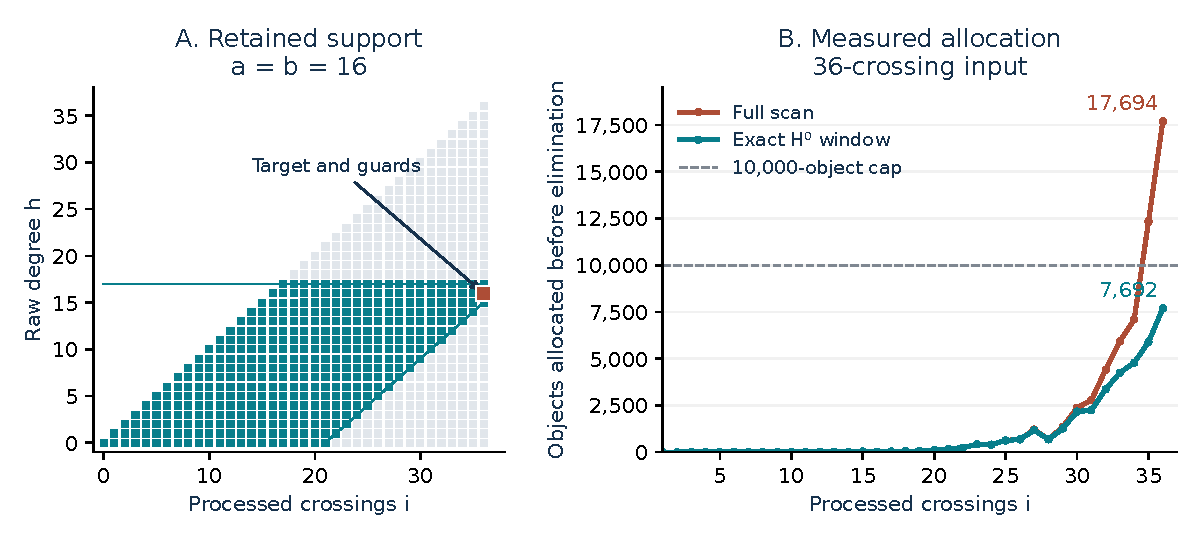
\includegraphics[width=\textwidth]{figures/window_support_and_profile.pdf}
\caption{Left: the exact moving support window for $n=36$ and target raw
degree $16$.  The guard degrees retain the incident differentials.
Right: actual pre-elimination allocations for the supplied stress diagram
under the same crossing order.  The 10,000-object ceiling is crossed by the
full scan and respected by the window scan.}
\label{fig:window-profile}
\end{figure}

\section{A finite perturbation method for exact minimal complexes}
\label{sec:perturbation-theory}

The window scanner reduces the portion of a complex that must be
constructed.  A complementary question is how to reduce a complex once it
exists.  This section separates scalar linear algebra from the remaining
cobordism calculation and derives a finite homological perturbation
algorithm.  The construction uses the established perturbation lemma
\cite{crainic}; the point here is an explicit nilpotence bound for the
implemented algebra, an exact multiplicity profile, and a checked
implementation of the resulting maps.

All objects below have the same current frontier with $w=2k$ endpoints.
They are loopless matchings, with raw homological placements retained and
the quantum grading forgotten.  The grading introduced next is an
intrinsic grading of the morphism algebra.  It is not the raw homological
degree and does not require the program to reconstruct the forgotten
quantum shifts.

\subsection{Positive grading without a Catalan frontier assumption}

For two matchings $a,b$, let $c(a,b)$ be the number of circle components in
the union of $a$ and a reversed copy of $b$.  The implemented morphism
basis consists of one canonical disk on each such circle, decorated with
zero or one dot.  This is the familiar dotted-cobordism and arc-algebra
description\cite{barnatan,khovanov_arc}.  A basis element carrying $d$
dots receives intrinsic degree
\begin{equation}
 \ell(a,b;d)=k-c(a,b)+2d.
 \label{eq:intrinsic-degree}
\end{equation}

The relevant matching family is the one occurring in the executed scan.
Its endpoints need not lie on one noose, and its matchings need not be
noncrossing with respect to their numerical labels.  Nevertheless the
spherical projection has a checkerboard face coloring.  Orient each edge
so that the black face is on its left.  At each crossing the four edge
directions alternate between incoming and outgoing, and either smoothing
joins incoming to outgoing.  At a fixed cut this gives a fixed division of
the frontier into $k$ positive and $k$ negative endpoints; every smoothing
matching joins opposite classes.

Thus the abstract disk gluings used below are oriented.  This is the
condition needed for the Euler-characteristic calculation, and it does
not require a Catalan count.  One should not instead declare every
unconstrained perfect matching on a labeled set admissible: for four
endpoints the three distinct pairings together need not admit the required
common endpoint orientations.  The present argument uses matchings
actually furnished by a spherical diagram.

\begin{lemma}[Homogeneous composition and degree range]
\label{lem:intrinsic-grading}
Every nonzero basis morphism has intrinsic degree in $[0,w]$.
Composition adds intrinsic degrees.  Degree zero consists precisely of
scalar identities between equal matchings.
\end{lemma}

\begin{proof}
Since $1\leq c(a,b)\leq k$ for a nonempty frontier and
$0\leq d\leq c(a,b)$,
\[
 0\leq k-c(a,b)+2d\leq k+c(a,b)\leq2k=w.
\]
At the empty frontier only the empty object and its scalar endomorphisms
remain, so the statement also holds for $w=0$.  Degree zero requires
$c(a,b)=k$ and $d=0$.  The union has $k$ two-edge circles exactly when
$a=b$, and the undotted canonical cobordism is then the identity.

For composition from $a$ through $b$ to $c$, abbreviate
$c_{ab}=c(a,b)$, $c_{bc}=c(b,c)$ and $c_{ac}=c(a,c)$.  Before reduction,
the composite surface has Euler characteristic
\begin{equation}
 \chi=c_{ab}+c_{bc}-k,
 \label{eq:composite-euler}
\end{equation}
because $k$ intervals of the middle matching are glued.  Let $d_{\rm in}$
be the total input dot count.  Replacing this surface by its canonical
output disks through neck cutting raises Euler characteristic by two for
each additional dot.  Accordingly every nonzero output monomial satisfies
\begin{equation}
 2d_{\rm out}=2d_{\rm in}+c_{ac}-\chi.
 \label{eq:dot-euler-balance}
\end{equation}
The factor two in this identity is essential.  A positive-genus component
contributes zero over $\mathbb F_2$ after handle reduction; double dots and
undotted spheres also vanish, while a dotted sphere evaluates to one.
These relations preserve the same degree balance whenever a term remains.
Therefore
\begin{align*}
 \ell_{\rm out}
 &=k-c_{ac}+2d_{\rm out}\\
 &=k-\chi+2d_{\rm in}\\
 &=2k-c_{ab}-c_{bc}+2d_{\rm in}
   =\ell_{\rm first}+\ell_{\rm second}.
\end{align*}
The calculation concerns abstract oriented surfaces, so numerical endpoint
order and the number of boundary components of the scanned region do not
enter it.
\end{proof}

Let $J$ be the ideal of positive intrinsic-degree morphisms.  For a finite
set $\mathcal M$ of distinct executed matchings, the basic algebra is
$A=\operatorname{End}(\bigoplus_{a\in\mathcal M}a)$.

\begin{corollary}[Uniform nilpotence]
\label{cor:radical-nilpotence}
One has
\[
 J^{w+1}=0,\qquad A/J\cong\prod_{a\in\mathcal M}\mathbb F_2.
\]
The same nilpotence exponent applies to matrices of arbitrary finite size
over this matching category.  In the additive closure, an object with
$m_a$ copies of each matching has endomorphism quotient
$\prod_a\operatorname{Mat}_{m_a}(\mathbb F_2)$, rather than a product of
one-dimensional fields.  The ideal $J$ is the radical of these
finite-dimensional algebras.
\end{corollary}

\begin{proof}
A product of $w+1$ positive-degree basis terms would have degree at least
$w+1$, where all morphism spaces vanish by
Lemma~\ref{lem:intrinsic-grading}.  Expand sums and matrix products into
composable paths to obtain the same conclusion for arbitrary matrix
sizes.  The degree-zero description gives the displayed quotients.  A
nilpotent ideal lies in the radical, while a semisimple quotient forces
the reverse containment here.
\end{proof}

\subsection{The scalar differential gives the exact remaining dimensions}

Let $(C,d)$ be a finite complex over this category.  Extract $d_0$ by
keeping only the undotted constant coefficient between equal matchings;
put $\delta=d+d_0$.  Every entry of $\delta$ lies in $J$.  Projection to
degree zero is compatible with composition, so $d^2=0$ implies
$d_0^2=0$.

For each matching $a$ and raw degree $h$, let $V_{a,h}$ be the vector space
of its copies in $C^h$.  The scalar differential forms independent binary
complexes
\[
 \cdots\longrightarrow V_{a,h-1}
 \xrightarrow{d_{0,a,h-1}}V_{a,h}
 \xrightarrow{d_{0,a,h}}V_{a,h+1}\longrightarrow\cdots.
\]
Define
\begin{equation}
 m_{a,h}=\dim V_{a,h}
          -\operatorname{rank}(d_{0,a,h-1})
          -\operatorname{rank}(d_{0,a,h}).
 \label{eq:scalar-minimal-profile}
\end{equation}

\begin{theorem}[Exact minimal multiplicity profile]
\label{thm:scalar-minimal-profile}
There exists a complex homotopy equivalent to $(C,d)$ whose differential
lies entirely in $J$ and which has exactly $m_{a,h}$ copies of matching
$a$ in degree $h$.  Every such minimal model has the same multiplicities.
Thus the number of remaining objects can be computed by binary linear
algebra before carrying out the nonlinear cobordism correction.
\end{theorem}

\begin{proof}[Construction of the scalar contraction]
In every binary complex choose decompositions
\[
 V_{a,h}=B_{a,h}\oplus H_{a,h}\oplus L_{a,h},
 \qquad
 B_{a,h}=\operatorname{im}d_{0,a,h-1},
\]
where $B_{a,h}\oplus H_{a,h}=\ker d_{0,a,h}$ and
$d_0:L_{a,h}\to B_{a,h+1}$ is an isomorphism.  Let
$H=\bigoplus_{a,h}a^{m_{a,h}}[h]$, using $[h]$ here only to record a raw
placement.  Let $i:H\to C$ include the chosen homology representatives,
$p:C\to H$ project along $B\oplus L$, and $h:C\to C$ take each boundary
back to its chosen preimage in $L$, vanishing on $H\oplus L$.

All these maps have scalar identity entries between equal matchings.  They
satisfy
\begin{equation}
 pi=1,\quad d_0i=0,\quad pd_0=0,\quad
 d_0h+hd_0=1+ip,\quad hi=0,\quad ph=0,\quad h^2=0.
 \label{eq:scalar-contraction-identities}
\end{equation}
The next theorem lifts this contraction to the full $d$ without changing
$H$ as an object.  Its resulting differential lies in $J$.  Uniqueness is
proved below.
\end{proof}

The program obtains $B$ from independent original image columns and $L$
from their corresponding source vectors.  It extends $B$ to a basis of
the kernel to choose $H$, and solves for coordinates in $B\oplus H\oplus L$.
This provides the actual maps in~\eqref{eq:scalar-contraction-identities},
not only the ranks in~\eqref{eq:scalar-minimal-profile}.

\subsection{A finite homological perturbation formula}

Composition is written in the conventional order: $fg$ means first $g$,
then $f$.  The code's composition helper takes its arguments in execution
order: the second map acts after the first.

\begin{theorem}[Finite lifted contraction]
\label{thm:finite-hpl}
Assume~\eqref{eq:scalar-contraction-identities}, let $d=d_0+\delta$ with
$d^2=0$, and suppose the entries of $\delta$ lie in $J$.  Define
\begin{align}
 F&=\sum_{j=0}^{w}(h\delta)^j=(1+h\delta)^{-1},&
 G&=\sum_{j=0}^{w}(\delta h)^j=(1+\delta h)^{-1},
 \label{eq:finite-series}\\
 i'&=Fi,& p'&=pG,& h'&=Fh=hG,\nonumber\\
 D&=p\delta Fi=pG\delta i.&&
 \label{eq:finite-hpl-maps}
\end{align}
These are finite sums, and $(H,D)$ is a minimal complex with a strong
deformation retraction from $(C,d)$.  Explicitly,
\begin{gather}
 D^2=0,\quad di'=i'D,\quad p'd=Dp',\quad p'i'=1,
 \label{eq:lifted-chain-identities}\\
 dh'+h'd=1+i'p',\qquad h'i'=0,\quad p'h'=0,\quad (h')^2=0.
 \label{eq:lifted-retraction-identities}
\end{gather}
The number of perturbation factors needed is at most $w$, independent of
the number of objects or the size of their scalar blocks.
\end{theorem}

\begin{proof}
The maps $i,p,h$ have intrinsic degree zero.  Therefore $h\delta$ and
$\delta h$ have entries in $J$, and
Corollary~\ref{cor:radical-nilpotence} proves the inverse identities in
\eqref{eq:finite-series}.  These are the standard perturbation formulas
\cite[Sections~2--3]{crainic}; a direct verification in characteristic two
is short enough to record.

Put $e=ip$ and
\[
 A=\delta F=G\delta.
\]
The finite series imply
\begin{equation}
 A=\delta+\delta hA=\delta+Ah\delta,
 \quad F=1+hA,\quad G=1+Ah.
 \label{eq:auxiliary-hpl-identities}
\end{equation}
There is also the identity
\begin{equation}
 d_0A+Ad_0=AeA.
 \label{eq:auxiliary-hpl-maurer}
\end{equation}
To verify it, multiply its left side by $1+\delta h$ on the left and
$1+h\delta$ on the right.  Using $AF^{-1}=\delta$ and
$G^{-1}A=\delta$ gives
\begin{align*}
 &(1+\delta h)(d_0A+Ad_0)(1+h\delta)\\
 &\quad=d_0\delta+\delta d_0
       +\delta(hd_0+d_0h)\delta\\
 &\quad=\delta^2+\delta(1+e)\delta=\delta e\delta.
\end{align*}
Here $d^2=0$ gives $d_0\delta+\delta d_0=\delta^2$ over
$\mathbb F_2$.  Multiplying by $G$ and $F$ proves
\eqref{eq:auxiliary-hpl-maurer}.

Now $D=pAi$, so
\[
 D^2=pAeAi=p(d_0A+Ad_0)i=0.
\]
Since $i'=i+hAi$, equations
\eqref{eq:scalar-contraction-identities} and
\eqref{eq:auxiliary-hpl-identities} give
\[
 di'=eAi+hd_0Ai=eAi+hAeAi=i'D.
\]
The same calculation on the other side gives $p'd=Dp'$.  Expanding
$p'i'=(p+pAh)(i+hAi)$ leaves only $pi=1$, by the three side conditions
$hi=ph=h^2=0$.

Finally $h'=h+hAh$.  Expand $dh'+h'd$ and use
$A=\delta+\delta hA=\delta+Ah\delta$ to cancel the terms containing a
single $\delta$.  What remains is
\begin{align*}
 dh'+h'd
 &=1+e+eAh+hAe+h(d_0A+Ad_0)h\\
 &=1+e+eAh+hAe+hAeAh=1+i'p'.
\end{align*}
Expanding $h'i'$, $p'h'$ and $(h')^2$ similarly makes every term contain
$hi$, $ph$ or $h^2$, so each vanishes.  Each term of $D=p\delta Fi$
contains a positive-degree factor $\delta$, hence $D$ lies in $J$ and is
minimal.
\end{proof}

\begin{lemma}[Uniqueness of minimal models]
\label{lem:minimal-uniqueness}
Two finite complexes with differentials in $J$ that are homotopy equivalent
are chain isomorphic.  Their multiplicities agree matching by matching and
raw degree by raw degree.  In particular, the multiplicities in
Theorem~\ref{thm:scalar-minimal-profile} agree with any exhaustive unit
cancellation result.
\end{lemma}

\begin{proof}
Reduce a homotopy equivalence and its inverse modulo $J$.  Both reduced
differentials are zero, so the homotopy equations say that the reduced
term maps are inverse in each degree.  Thus the binary multiplicity spaces
agree.  Each lifted composite differs from the identity by a matrix in
$J$.  Such a matrix is inverted by a finite geometric series of length
at most $w+1$.  Consequently each original term map is invertible; its
inverse commutes with the differential because the term map does.  This
gives a chain isomorphism.  The assertion concerns multiplicities and
isomorphism type, not a canonical displayed basis or identical matrices.
\end{proof}

\subsection{What the implementation checks}

The research module \texttt{perturbation.py} first constructs the scalar
contraction, then computes $i'$ by repeatedly applying $h\delta$ to its
current term.  It obtains $D$ from $p\delta i'$.  With certification enabled
it also constructs $p',h'$ and verifies all identities in
\eqref{eq:lifted-chain-identities}--\eqref{eq:lifted-retraction-identities},
together with the original $d^2=0$, over the same exact cobordism algebra
used by the scanner.  It checks the finite-series termination and the
absence of scalar units in the output differential.

The corrected maps are stronger evidence than an agreement of final ranks:
they give the explicit homotopy equivalence needed for continuing the scan.
Because planar extension preserves homotopies, an installed model can be
extended through subsequent crossings.  The test suite compares its
matching-and-degree multiplicities with exhaustive scalar cancellation at
intermediate prefixes, checks final homology independently, and confirms
that a corrupted contraction map is rejected.  An additional independent
grading audit examined all bipartite matching monomial products through
six endpoints, including the non-Catalan six-endpoint matching: all 3533
products and 1576 nonzero output monomials obeyed
Lemma~\ref{lem:intrinsic-grading}.

\subsection{Cost, useful regimes, and remaining obstruction}

Write $N$ for the input object count at one stage and $H=\sum_{a,h}m_{a,h}$
for the output count.  There are at most $2^{w/2}$ dot-mask coefficients in
one morphism.  Scalar contraction uses binary matrices with at most $N$
rows and columns and therefore has polynomial bit cost, with a standard
cubic bound sufficient here.  The inclusion series performs at most $w$
iterations on matrices of size at most $N$ by $H$.  A conservative bound
for the reduction without optional certificates is
\begin{equation}
 O\bigl(N^3+(w+1)N^2(H+1)\,2^{O(w)}\bigr).
 \label{eq:hpl-cost}
\end{equation}
Computing and verifying all contraction maps has the coarser bound
\[
 O\bigl((w+1)(N+1)^3\,2^{O(w)}\bigr).
\]
These estimates allow dense maps; sparsity can help but is not assumed.
They follow by counting ordinary matrix-composition paths and charging
$2^{O(w)}$ for a cobordism product and its bit operations.  Cache storage
and dictionary bookkeeping remain polynomial in $N$ times $2^{O(w)}$.

The attraction is most pronounced when the scalar differential has large
rank, so $H\ll N$.  In the extreme $H=0$, scalar acyclicity already implies
full contractibility: the corrected inclusion and reduced differential
have empty source.  If an explicit contracting homotopy is requested, its
construction still has a cost.  When scalar cancellation is sparse and
cheap, assembling a global binary decomposition and dense corrected maps
can instead add overhead.  Thus no pointwise or asymptotic speed advantage
over the existing scalar scanner is claimed.  The experiment section
reports the measured regimes, including the distinction between natural
knot complexes and synthetic algebraic blocks.

This method does not control $N$ or $H$ by frontier width alone.  It
computes the minimal multiplicity profile of an already represented
complex, and an explicit output must still list its $H$ objects.  Known
fixed-braid-width exponential examples therefore remain an obstruction to
a universal explicit-basis complexity theorem.  The finite perturbation
bound supplies a precise local reduction cost and a certificate; combining
it with window bounds or a separate structural compression theorem is the
remaining route to stronger global guarantees.

\section{A deterministic near-linear terminal boundary-pattern algorithm}
\label{sec:terminal-patterns-new}

The previous terminal implementation in report 06 tests all sets of at most
three primal edges and traverses the remaining graph for each set.  Its
$O(E^4)$ worst-case bound can be improved to $O(s_P\log(s_P+2))$ deterministic
word-RAM operations, where $s_P=2E$ is the number of darts.  The improvement is
an implemented graph algorithm with an independently checked negative
certificate.  It does not require a generic four-connectivity routine.
This is an algorithmic consequence of the established theory of essential
boundary patterns, rather than a new topological characterization.

\subsection{Input and topological precondition}

The ambient manifold is a known 3-ball $B$.  Its boundary pattern $P$ is a
disjoint union of embedded trivalent multigraphs and vertex-free circles.
The input contains a cyclic triple at each graph vertex.  Dart $2e$ is
paired with dart $2e+1$ by the fixed-point-free involution
$\alpha(d)=d\mathbin{\mathrm{xor}}1$.  Write $\sigma$ for the permutation
whose cycles are the supplied triples.  The face walks are the cycles of
$\phi=\sigma\alpha$.

The implementation checks that the dart list is exactly a permutation of
$\{0,\ldots,s_P-1\}$, that every vertex has degree three, and that
$V_i-E_i+F_i=2$ for every connected graph component.  Thus each connected
rotation system has a spherical embedding.  A rotation system does not
specify the relative nesting of distinct graph components.  This omission
does not affect the essentiality decision: any pattern with two or more
components is inessential, independently of their nesting.

The supplied assertion that the ambient manifold is a 3-ball remains a
precondition.  In particular, a spherical boundary does not by itself
establish this precondition.  The routine does not decide whether an
arbitrary 3-manifold is a ball.

\subsection{The dual triangle criterion}

Recall that a pattern on a ball is essential when every transverse simple
closed curve meeting $P$ at most three times bounds a boundary disc whose
intersection with $P$ is empty, a single arc, or a single tripod.
Lackenby's Proposition 2.6 \cite{lackenby2026} characterizes this property using the planar
dual and four-connectivity.  We use the following equivalent form.

\begin{theorem}[Terminal dual triangle criterion]
\label{thm:terminal-triangle}
Let $P$ be a nonempty connected trivalent graph embedded in a sphere, and
let $G$ be its embedded dual, with loops and multiple edges retained.
Then the pattern is essential if and only if:
\begin{enumerate}
\item $G$ has no loops;
\item $G$ has no two distinct edges with the same pair of endpoints;
\item every three-cycle of $G$ is the boundary of a face of $G$.
\end{enumerate}
The complete patterns consisting of the empty set or one vertex-free
circle are also essential.  Every disconnected nonempty pattern is
inessential.
\end{theorem}

\begin{proof}
We use the elementary bond--cycle duality for connected sphere-embedded
graphs: a minimal nonempty primal edge cut is dual to a simple dual cycle,
and conversely.  One way to see this is to thicken either side of a
minimal edge cut and fill the complementary discs containing no vertices
on the other side.  Connectedness on both sides leaves one boundary
curve, crossing exactly the cut edges.  Its arcs through the primal
faces give the dual cycle.  Conversely, a simple dual cycle is a Jordan
curve; its two sides give connected primal vertex sets and hence a
minimal edge cut.  Loops and pairs of parallel dual edges correspond to
cuts of size one and two, respectively.

An edge cut of size one or two gives a violating boundary curve.  A
three-edge bond is harmless precisely when one side has a single primal
vertex: the boundary disc then meets the trivalent graph in a tripod.
In the dual, this is precisely the condition that its three-cycle is
facial.  Thus every obstruction in (1)--(3) gives a violating curve.

For completeness, suppose that (1) and (2) hold.  Bond--cycle duality
implies that the primal graph has no edge cut of size one or two.  Let
$\gamma$ be a simple closed curve meeting the graph in $k\leq3$ points.
If one side contains no primal vertex, its intersection with the graph
is either empty or, when $k=2$, a single arc; that side is allowed.
Otherwise let $U$ be the vertices on one side.  The edge boundary
$\delta(U)$ has at most $k$ edges.  Since smaller edge cuts do not exist,
$|\delta(U)|=k=3$, and $\gamma$ crosses each of these three edges exactly
once.  The induced graphs on $U$ and on its complement are connected:
two components on one side would each have at least three outgoing
edges, exceeding the available three.  Thus $\delta(U)$ is a
three-edge bond.  By (3), its dual triangle is facial, so one side has a
single primal vertex and is an allowed tripod disc.  This proves
essentiality.

The empty pattern and a sole circle satisfy the definition directly.
When a pattern is disconnected, there is a separating curve disjoint
from it with nonempty pattern on both sides.  This is violating.
\end{proof}

The face occurrence convention matters at the smallest input.  For
$G=K_3$, its unique three-cycle bounds two different faces.  The primal
pattern is the theta graph, with two tripod sides, and is essential.
The implementation records two facial occurrences and one distinct
facial vertex triple.  It accepts the triangle when at least one facial
occurrence exists.  The $K_4$ exception is handled in exactly the same
way, with four distinct facial triples.

\subsection{Algorithm and complexity}

After validation and the disconnected, empty, and circle cases, construct
each dual edge as $(f(d),f(\alpha(d)),e)$, where $f(d)$ is the face
containing dart $d$.  Sorting these triples detects loops and repeated
endpoint pairs.  Once the dual is simple, the three faces around each
primal vertex form a facial triangle of the dual; retain these triples,
sorted with multiplicity.

Every nonempty subgraph of a simple planar graph has a vertex of degree
at most five.  Delete such vertices successively.  A queue implementation
adds a vertex initially if its degree is at most five, or later when its
degree first falls from six to five.  Thus every vertex is queued once
and every edge is examined a constant number of times.

Orient each edge from its earlier-deleted endpoint to its later-deleted
endpoint.  There are at most five forward neighbors at every vertex.
For each unordered pair of forward neighbors, use binary search in the
sorted edge list to decide whether the pair completes a triangle.  A
triangle is encountered exactly once, at its earliest-deleted vertex.
Use a second binary search in the list of facial triples to decide
whether the triangle is facial.

\begin{theorem}[Implemented terminal complexity]
\label{thm:terminal-complexity}
For a valid input with $s_P$ darts, the classifier uses
$O(s_P\log(s_P+2))$ deterministic word-RAM operations and $O(s_P)$ words of
space.  Its triangle scan examines at most $10|V(G)|$ candidate neighbor
pairs.  All labels are dense integers of $O(\log(s_P+2))$ bits; a conservative
charge of this many bit operations per word operation gives
$O(s_P\log^2(s_P+2))$.  The separately supplied circle count also contributes
its own binary input length.
\end{theorem}

\begin{proof}
Validation, face traversal, dual construction, and degree peeling take
linear time apart from sorting.  All edge and face lists have $O(s_P)$
entries, so sorting costs $O(s_P\log(s_P+2))$.  Each of the $|V(G)|$ vertices
contributes at most $\binom{5}{2}=10$ candidate pairs.  Each candidate
uses a constant number of binary searches and therefore
$O(\log(s_P+2))$ comparisons.  A returned negative certificate requires one
additional primal traversal and sorting its two vertex lists, again
within the stated bound.  Every stored list has linear size.
\end{proof}

No hash-table assumption enters this bound.  The implementation uses
sorted edge and face arrays and a queue.  The degree peeling does not
search for a minimum-degree vertex; any available vertex of degree at
most five suffices.

\subsection{Certificates and independent verification}

The three connected negative certificate kinds are a dual loop, a dual
bigon, and a nonfacial dual triangle.  A certificate records the cyclic
list of dual vertices, the crossed primal edge labels, and the two
primal vertex sets obtained by deleting these edges.  A separate
verifier checks all labels, traverses the primal graph after deleting
the indicated edges, and confirms that the edge boundary of one side
is exactly the indicated set.  For three edges it also checks that
both sides contain more than one vertex.  Thus the verifier does not
rerun the triangle enumeration.

These data determine a violating curve on the known boundary sphere:
join consecutive crossings within their specified primal face.  Pushing
one boundary disc slightly into the ball gives a violating properly
embedded disc.  The disconnected certificate establishes existence of
a zero-intersection violating curve; without relative nesting data it
does not specify a particular geometric representative.

A terminal witness is not yet a normal compression disc in the original
knot exterior.  Transporting it backwards through a hierarchy still
requires the cut surfaces, boundary identifications, and changes made
during parallelity-bundle simplification.  The present improvement
removes repeated small-cut enumeration at the terminal stage; it does
not supply those geometric operations.

\subsection{Validation and reproducible comparison}

The tests compare the new classifier and its certificates against the
unmodified report-06 bond enumerator.  The small-map test exhausts all
$15+10395=10410$ pairings of darts at two and four cyclically ordered
trivalent vertices.  Of these, 5628 have spherical graph components
and 4782 are rejected as non-spherical.  Every accepted input is checked
against the old classifier; every returned connected negative
certificate is also translated into the old verifier's primal-bond
format and checked there.

Additional tests use random larger ribbon maps, sphere triangulations
generated by stellar subdivisions and legal edge flips, relabeling and
mirroring, malformed inputs, corrupted witnesses, all three obstruction
types, the $K_3$ double-face case, and an essential pattern with 60000
darts.  The deterministic benchmark compares complete calls from a
prepared JSON-like input through validation to the returned result.
Fixture construction and external JSON reading/writing are excluded
from both timings.

The full raw timing records, machine description, source provenance,
and generator parameters are included in the accompanying artifacts.
They measure this terminal subroutine and do not establish a running-time
bound for a complete hierarchy-based unknot recognizer.


\begin{figure}[H]
\centering
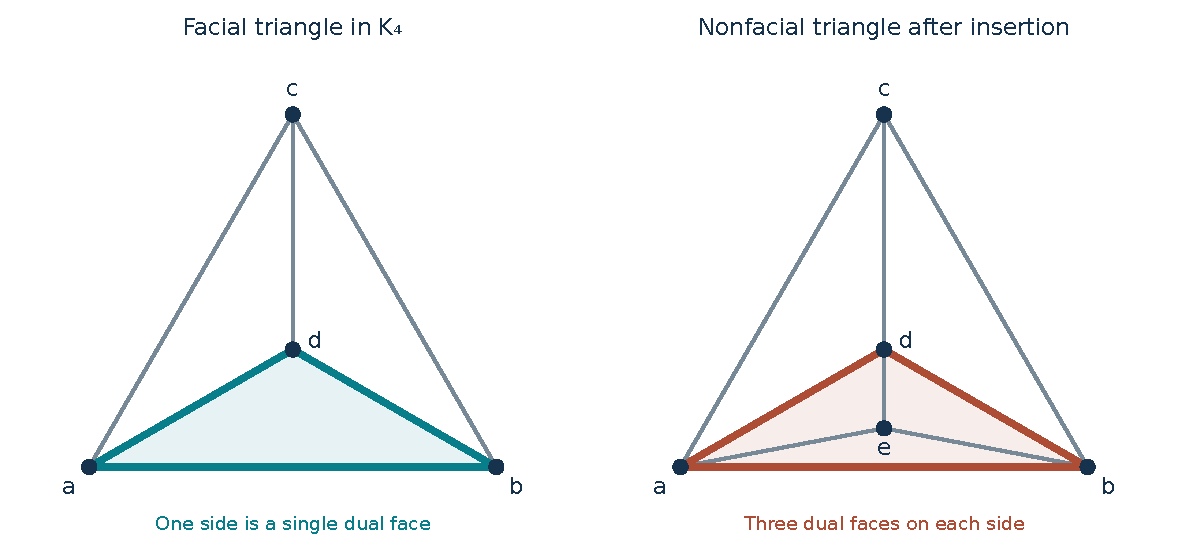
\includegraphics[width=0.93\textwidth]{figures/terminal_triangle.pdf}
\caption{The dual criterion on explicit sphere triangulations.  A facial
triangle in $K_4$ is harmless.  Inserting a vertex into that face makes its
old boundary a nonfacial triangle: the two sides contain three primal
vertices each, producing a three-edge violating bond.}
\label{fig:terminal-dual}
\end{figure}

\section{An output-size obstruction for compressed cuts}
\label{sec:compressed-cut-output}

An efficient compressed cutting theorem must be translated into an
explicit output contract.  Merely storing normal coordinates in binary
does not make an expanded component list efficient.

\begin{proposition}[Parallel-disc output lower bound]
\label{prop:parallel-disc-output}
There is a fixed one-tetrahedron triangulated 3-ball and a family of
properly embedded orientable normal surfaces $S_W$, for integers $W\ge1$,
with normal-coordinate input length $O(\log(W+1))$, such that cutting
along $S_W$ produces $W+1$ connected components.  Between successive
normal discs are $W-1$ pairwise disjoint product slabs.  Consequently an
algorithm that explicitly lists all cut components, or all these
individual product slabs, requires $\Omega(W)$ output operations.
\end{proposition}

\begin{proof}
Choose a vertex of one tetrahedron and take $W$ pairwise disjoint,
nested, normally isotopic triangles linking that vertex.  Their normal
vector has one coordinate $W$ and six zero coordinates.  Each triangle
is a properly embedded disc.  In a collar of one such disc, the
successive triangles divide the collar into $W-1$ copies of
$D^2\times I$.  The two remaining regions, one towards the vertex and
one away from it, are also balls.  Therefore the cut manifold has
$W+1$ components.  Writing one record for each component or slab has
the asserted lower bound.  Taking $W=2^k$ makes this exponential in
the binary coordinate length.
\end{proof}

This does not contradict a compressed-cutting theorem.  It shows that
its concrete interface must support aggregated multiplicities,
symbolic families, or a stated connectedness restriction.  A suitable
record for this example is one ordinary product type with binary
multiplicity $W-1$, together with the two exceptional end regions.
It is insufficient to advertise polynomial time in $\log W$ while
returning a Python list with one element per product region.

More generally, if $S$ is a connected two-sided normal surface with
normal vector $v$, then $Wv$ is represented by $W$ parallel copies of
$S$.  With compatible collar markings,
\[
 M\mathbin{\backslash\!\backslash}(WS)
 \cong
 \bigl(M\mathbin{\backslash\!\backslash}S\bigr)
 \sqcup
 \coprod_{i=1}^{W-1}(S\times I).
\]
Thus multiplicity extraction can be an exact preprocessing operation
when connectedness and two-sidedness of the base surface are certified.
Dividing coordinates by their greatest common divisor alone does not
certify either condition.  For a one-sided connected surface, doubling
its normal vector describes the boundary of a regular neighborhood,
which can be connected; blindly interpreting that factor of two as
two disjoint copies would be incorrect.

In the July 2026 hierarchy paper, Theorem 14.4 (p.~51) gives the
compressed cut information, whereas Proposition 14.2 (p.~50) adds
essential-pattern and irreducibility hypotheses for the subsequent
simplification.  These are different contracts.  In particular,
an undecided unknot exterior does not supply an essential initial
pattern as an available assumption.  The representation lower bound
above is an implementation obligation, not an assertion that the
literature's compressed theorem is false.

\section{Quantitative accounting for a future hierarchy engine}
\label{sec:hierarchy-accounting}

The near-linear terminal test removes one repeated search from the
hierarchy route.  To obtain a general quasi-polynomial recognizer, one
must also bound the construction and revision of the hierarchy, the
size of its compressed states, and the cost of transporting a terminal
witness.  This section specifies a sufficient global accounting theorem.
It does not assert that the geometric hypotheses have been established
for the delivered implementation.

\subsection{The precise status of the source bounds}

The February 2021 slides cited here, the file
\code{quasipolynomial-talk.pdf}, announce
$n^{O(\log n)}$ \cite{lackenbytalk}.  The November 2024 Tsinghua abstract
announces
\[
 2^{O((\log n)^3)}=n^{O((\log n)^2)}
 \qquad\cite{lackenby2024}.
\]
These are different stated bounds.  Both are quasi-polynomial, and the
sources reviewed here do not establish an explanation for the difference.
The July 2026 preprint is a separate source: it gives a hierarchy
algorithm and efficient certificate operations, while identifying further
speed-up as future work \cite{lackenby2026}.

For its iteration analysis, let $L$ bound the length of every hierarchy
that occurs, and let $g$ bound every nonnegative complexity digit that
is stored, including after a suffix is rebuilt.  Proposition~9.1 gives
\begin{equation}
 \#\{\hbox{executions of any fixed algorithmic step}\}
 \leq L(g+1)^L.
 \label{eq:lackenby-iteration-bound}
\end{equation}
Proposition~10.2 gives the refined length bound
$L\leq4c_q(\mathcal H)$, in terms of the initial handle structure's
q-complexity.  For a linear-size initial structure of uniform type this
is $L=O(n)$ \cite[Props.~9.1 and 10.2]{lackenby2026}.

Equation~\eqref{eq:lackenby-iteration-bound} is not yet a bit-time estimate.
Its digits concern pattern complexity, including intersections with the
boundary pattern, rather than genus alone.  A bound valid only for the
first chosen surfaces is insufficient when later replacements introduce
new surfaces.  Moreover, each counted step may act on a compressed object
whose bit length must itself be controlled.

Even if the additional estimate $g\leq(n+2)^a$ were supplied, combining it
only with $L=O(n)$ would give the coarse iteration bound
$\exp(O(n\log(n+2)))$.  This is not a quasi-polynomial upper bound.
It is also not a lower bound on the algorithm: a sharper analysis may
exploit correlations between successive choices or long stretches of
forced operations.  The distinction motivates the following elementary
accounting result.

\subsection{A rooted-tree bound that includes forced operations}

All logarithms in this subsection are natural logarithms.  A rooted tree
represents \emph{actual execution occurrences}: distinct visits are
distinct nodes unless a separate memoization argument proves that they
can be charged to one computation.  At a node $v$, write $b(v)$ for the
number of its children.  A node with one child describes a forced
operation and contributes $\log b(v)=0$.  Leaves contribute no logarithm.

\begin{theorem}[Depth and cumulative branching]
\label{thm:hierarchy-tree-accounting}
Let $T$ be a rooted, finitely branching tree of depth at most $D$, where
depth counts edges.  Suppose that every root-to-leaf path satisfies
\begin{equation}
 \sum_{\substack{v\ \mathrm{on\ the\ path}\\b(v)>0}}\log b(v)\leq B.
 \label{eq:branch-budget}
\end{equation}
Then
\begin{equation}
 |V(T)|\leq(D+1)e^B.
 \label{eq:tree-node-bound}
\end{equation}
If all work associated with one node has bit cost at most $C$, including
its assigned state construction, tests, certificate data, and transition
work, the total assigned cost is at most $C(D+1)e^B$.
\end{theorem}

\begin{proof}
Finite branching and bounded depth imply that $T$ is finite.  Assign the
root weight $1$, and assign every child of an internal node $v$ the
weight of $v$ divided by $b(v)$.  Thus at every fixed depth the sum of
the node weights is at most $1$: passing to the next depth preserves the
weight at internal nodes and drops the weight at leaves.

For a node $u$, its weight is
\[
 p(u)=
 \prod_{\substack{v\ \mathrm{a\ proper}\\\mathrm{ancestor\ of}\ u}}
 \frac1{b(v)}.
\]
Extend its path to a leaf.  Since every summand in
\eqref{eq:branch-budget} is nonnegative, the ancestor sum for $u$ is at
most $B$.  Hence $p(u)\geq e^{-B}$.  If there are $N_j$ nodes at depth
$j$, then $N_je^{-B}\leq1$, so $N_j\leq e^B$.  Summing over
$j=0,\ldots,D$ proves~\eqref{eq:tree-node-bound}.  Summing the stated
per-node costs proves the final assertion.
\end{proof}

The weights are a counting device.  No randomized algorithm or
probabilistic running-time assumption is involved.  The same proof works
with computable bounds $\widehat b(v)\geq b(v)$ in place of the actual
positive child counts: distribute weight $p(v)/\widehat b(v)$ to each
child, so that total weight can only decrease.

Unary chains explain why the depth term cannot be omitted.  A chain of
$D+1$ nodes has $B=0$ and attains the bound exactly.  Conversely, a
small bound on the length of each completed geometric hierarchy is not
automatically a bound on $D$: rebuilding its suffix many times can
create many execution occurrences.  A tree interpretation must account
for those occurrences explicitly.

\begin{corollary}[Explicit quasi-polynomial budgets]
\label{cor:hierarchy-qp-budget}
Suppose a complete algorithm on $n$-crossing inputs admits the accounting
of Theorem~\ref{thm:hierarchy-tree-accounting}, uniformly over all its
inputs and executions.  If
\[
 B(n)+\log(D(n)+1)+\log(C(n)+1)
     =O\bigl((\log(n+2))^r\bigr)
\]
for a fixed $r\geq1$, then its accounted bit time is
$\exp(O((\log(n+2))^r))$.
In particular, polynomial $C,D$ and
$B=O(\log^2(n+2))$ imply $n^{O(\log(n+2))}$ time; replacing that
branching budget by $O(\log^3(n+2))$ gives
$n^{O((\log(n+2))^2)}$.
\end{corollary}

\begin{proof}
Take logarithms of the time bound in
Theorem~\ref{thm:hierarchy-tree-accounting} and substitute the hypotheses.
\end{proof}

For example, polynomially many forced operations along a path are
compatible with the stronger bound when at most $O(\log n)$ nodes
branch and each has at most $n^{O(1)}$ children.  Their cumulative
branching is $O(\log^2 n)$.  If polynomial branching occurs at
$O(\log^2 n)$ levels instead, the same arithmetic gives
$O(\log^3 n)$.  These are sufficient accounting regimes, not an
explanation of the historical announcements.

This formulation permits the available choices to depend on the entire
earlier history.  It can therefore be more informative than multiplying
independent worst-case caps at every hierarchy level.  Nevertheless,
the bound must hold on all explored paths, including failed choices and
restarts.  A bound on one successful certificate, or on the number of
distinct unlabeled states, does not establish the hypotheses.

\subsection{The geometric obligations behind the symbols}

There are three distinct representation issues.  First, a polynomial
number of local handle types does not bound the number of handles.
Second, large normal coordinates require binary arithmetic and
multiplicity-aware output, as
Proposition~\ref{prop:parallel-disc-output} demonstrates.  Third, a
compact object can still require a costly search to construct.
The per-node bound $C$ must include all three issues rather than treating
surface production or witness transport as an oracle.

Theorem~14.4 of the 2026 paper supplies compressed cutting data in time
polynomial in the handle count and logarithm of the extended surface
weight.  Proposition~14.2's subsequent simplification has additional
irreducibility and essential-pattern hypotheses
\cite[Prop.~14.2 and Thm.~14.4]{lackenby2026}.
The latter hypothesis cannot be silently supplied by an undecided knot
exterior with empty initial pattern.  A verifier may establish it from
an appropriate certificate; a general producer must also handle the
opposite case.

A concrete realization of Corollary~\ref{cor:hierarchy-qp-budget} should
therefore attach to every state an encoding-size bound, an explicit
description of its admissible continuations, and a record of each
operation used to transfer boundary curves.  If a simplification is
conditional on essentiality, its contract must state how that
precondition is certified or how a compression witness is handled.
All outer changes of Heegaard data and all reconstructions of discarded
suffixes must receive a charge in the same execution accounting.

Efficient verification of a supplied hierarchy and efficient generation
of one are separate requirements.  The present package advances the
terminal test and the algebraic route, and gives exact interfaces against
which a hierarchy implementation can be audited.  It does not supply
uniform geometric bounds for $B,D,C$.  Proving those bounds, together
with an executable producer satisfying their hypotheses, remains the
step needed for a general hierarchy-based complexity theorem.

\section{Measurements, validation, and repository integration}
\label{sec:experiments}

The experiments separate three computational questions.  The window
benchmark measures the cost of obtaining a selected obstruction instead
of all homology.  The perturbation benchmark computes the same complete
homology by two reduction engines.  The pattern benchmark compares two
classifiers for an already known ball.  A speed ratio from one question
is not an end-to-end speed ratio for the other two.

All stored measurements use Python 3.12.14 on an x86-64 Linux environment
with glibc 2.39.  Raw repetitions, input diagrams or deterministic fixture
generators, crossing orders where applicable, and operation counts are
included.  Wall times are observations on this environment.  The paired
protocol reduces some variability but does not remove shared-machine
scheduling noise, especially for millisecond inputs.  Asymptotic claims
in this paper follow from the preceding proofs, rather than fits to these
small timing samples.

\subsection{Exact windows: less construction, sometimes an earlier verdict}

The window experiment uses one warmup per variant and seven timed pairs,
alternating which variant runs first.  Both variants receive identical
PD data and the same preselected crossing order.  Both use the baseline's
automatic shape-cache policy.  Diagram loading, order selection, and
cheap invariant filters are excluded.  The window orientation is fixed
for each row: the bound-aware automatic mirror selector is available to
callers but is not being credited for these measurements.

\begin{table}[htbp]
\centering\small
\setlength{\tabcolsep}{4pt}
\begin{tabular}{lrrrrr}
\toprule
Input & $n$ & Full (ms) & Window (ms) & Full/window & $\dim H^0$ \\
\midrule
Conway & 11 & 7.202 & 7.089 & 1.016 & 10 \\
Kinoshita--Terasaka & 11 & 8.954 & 7.747 & 1.156 & 10 \\
Hard unknot & 8 & 1.626 & 1.364 & 1.193 & 2 \\
Determinant-one grid & 10 & 4.826 & 1.455 & 3.316 & 2 \\
Mixed 5-braid & 36 & 904.254 & 581.562 & 1.555 & 698 \\
Conway, mirrored & 11 & 13.823 & 13.456 & 1.027 & 10 \\
K--T, mirrored & 11 & 13.184 & 14.254 & 0.925 & 10 \\
$T(4,7)$ control & 21 & 77.047 & 9.280 & 8.303 & 2 \\
$T(2,31)$ control & 31 & 11.580 & 6.467 & 1.791 & 2 \\
\bottomrule
\end{tabular}
\caption{Scanner-kernel medians from seven alternating pairs after a warmup of each variant. The window computes only normalized degree zero, while the full scan computes every degree. Input preparation and order selection are excluded.}
\label{tab:window-times}
\end{table}

\begin{table}[htbp]
\centering\small
\setlength{\tabcolsep}{4pt}
\begin{tabular}{lrrc}
\toprule
Input & Full peak & Window peak & Window rejects unknot? \\
\midrule
Conway & 246 & 124 & Yes \\
Kinoshita--Terasaka & 246 & 118 & Yes \\
Hard unknot & 11 & 11 & No \\
Determinant-one grid & 54 & 24 & No \\
Mixed 5-braid & 17,694 & 7,692 & Yes \\
Conway, mirrored & 246 & 128 & Yes \\
K--T, mirrored & 246 & 122 & Yes \\
$T(4,7)$ control & 210 & 40 & No \\
$T(2,31)$ control & 186 & 66 & No \\
\bottomrule
\end{tabular}
\caption{Peak physical objects allocated before elimination. These are object counts, not peak resident-memory measurements. A degree-zero dimension of two is inconclusive.}
\label{tab:window-objects}
\end{table}


The most useful case is the repository's 36-crossing mixed five-braid
stress diagram.  Its complete unreduced rank is 5898, while its normalized
degree-zero rank is 698.  Thus this one degree already proves
nontriviality.  The median full scan took $0.904254$ seconds and the
window took $0.581562$ seconds, a ratio of approximately $1.55$.
The peak allocated objects decreased from 17694 to 7692, a reduction of
about $56.5\%$.  Figure~\ref{fig:window-profile} plots every allocation
stage, including the large final expansion.

The identical-cap experiment is more informative than a small timing
difference.  With a 10000-object ceiling the full scan raises
\texttt{ScanLimit} before allocating 17694 objects, while the window
completes with peak 7692 and returns the 698-dimensional obstruction.
This is a reproducible change in which exact question can be answered
within a stated resource limit.  The cap is an object cap, not a measured
resident-memory limit; morphisms, dictionaries and caches also use space.

Conway and Kinoshita--Terasaka both have degree-zero dimension 10 in these
conventions, so their window results are also decisive.  Their short wall
times should not be overinterpreted: the mirrored Kinoshita--Terasaka row
is slower with the window.  Truncation incurs bookkeeping, and different
remaining objects can change the pivot order.

The hard unknot, determinant-one grid knot, and torus controls all have
degree-zero dimension 2.  Those window results are inconclusive.  In
particular, the large ratio on the $T(4,7)$ control does not constitute
a faster complete recognition result: additional homology or a cheap
invariant still supplies nontriviality.  The standard recognition pipeline
already dispatches many of these inputs before Khovanov computation.
These rows deliberately isolate the scanner operation.

The saved JSON also contains the isolated-guard pruning ablation.  Every
ablation agrees on the requested ranks.  Its allocation profile explains
what this additional operation deletes, but the ablation was not timed
and no speed ratio is assigned to it.  For the final stress stage the
retained allocation is 7692; unit elimination and the valid deletion of
isolated guards leave the requested 698 objects.

\subsection{Perturbation: an exact prototype with a measured tradeoff}

The second experiment uses five warmed alternating pairs.  The complete
scanner and perturbation backend receive the same fixed crossing order,
with shape caching disabled in both.  They agree on the full homological
rank distribution for every row.  Optional construction and verification
of all contraction maps is excluded from the timing and tested separately.

\begin{table}[htbp]
\centering\small
\setlength{\tabcolsep}{4pt}
\begin{tabular}{lrrrr}
\toprule
Input & $n$ & Scalar (ms) & Perturbation (ms) & Scalar/pert. \\
\midrule
Hard unknot & 8 & 2.299 & 3.479 & 0.661 \\
Conway & 11 & 7.858 & 15.080 & 0.521 \\
Kinoshita--Terasaka & 11 & 8.572 & 19.468 & 0.440 \\
$T(3,7)$ & 14 & 13.637 & 15.951 & 0.855 \\
$T(4,7)$ & 21 & 45.236 & 60.884 & 0.743 \\
\bottomrule
\end{tabular}
\caption{Full Khovanov scans: five warmed alternating pairs, fixed order, shape cache disabled in both backends. The perturbation backend is slower on every natural input tested.}
\label{tab:hpl-natural}
\end{table}


The current perturbation implementation loses on every natural diagram
in Table~\ref{tab:hpl-natural}.  The extra binary basis construction and
map assembly outweigh the avoided individual cobordism operations in
these cases.  This is a reason to retain it as an explicit research
backend, and to use its rank profiles and certificates to design a
selective hybrid, rather than replace the default elimination routine.

There is nevertheless a regime where the construction has a concrete
advantage.  Consider two-term algebraic complexes with differential
\[
 d=I+xR\quad\text{over }\mathbb F_2[x]/(x^2),
\]
where $R$ is a deterministic pseudorandom binary matrix.  The scalar
differential is the identity, so its homology vanishes.  Moreover
$(I+xR)^2=I$, making full contractibility immediate.  These are valid
complexes over the one-arc endomorphism algebra, although no claim that
they arise from knot diagrams is made.

\begin{table}[htbp]
\centering\small
\setlength{\tabcolsep}{4pt}
\begin{tabular}{rrrrr}
\toprule
$R$ order & Objects & Scalar (ms) & Perturbation (ms) & Scalar/pert. \\
\midrule
16 & 32 & 0.162 & 0.192 & 0.842 \\
32 & 64 & 0.744 & 0.444 & 1.676 \\
64 & 128 & 4.022 & 1.449 & 2.776 \\
128 & 256 & 29.020 & 5.822 & 4.984 \\
256 & 512 & 204.609 & 31.587 & 6.478 \\
\bottomrule
\end{tabular}
\caption{Synthetic two-term complexes with differential $I+xR$ over $\mathbb F_2[x]/(x^2)$. These are algebraic stress tests, not knot diagrams. Both timings include construction of the same input complex.}
\label{tab:hpl-synthetic}
\end{table}


At matrix order 256, the median decreases from $0.204609$ to $0.031587$
seconds, about $6.48$ times.  Both timings construct the same input.
The scalar path performs many nilpotent updates; the perturbation path
detects scalar acyclicity and returns an empty minimal object.  Requiring
an explicit contracting homotopy would add work.  The benefit therefore
supports a specific implementation hypothesis---large scalar rank can
make block reduction attractive---without supplying an end-to-end
unknot speedup.  The stored small stress cases do check the complete
contracting identities.

\subsection{Terminal patterns: a large improvement in a narrow subroutine}

\begin{table}[htbp]
\centering\small
\setlength{\tabcolsep}{4pt}
\begin{tabular}{rrrr}
\toprule
Darts & New (ms) & Report 06 (ms) & Old/new \\
\midrule
24 & 0.062 & 2.526 & 40.6 \\
48 & 0.081 & 25.605 & 315.9 \\
72 & 0.108 & 152.797 & 1416.0 \\
96 & 0.149 & 487.551 & 3265.9 \\
144 & 0.166 & 2745.396 & 16517.9 \\
192 & 0.440 & 9530.512 & 21650.6 \\
\bottomrule
\end{tabular}
\caption{Known-ball terminal classifier: medians of three complete calls including validation. The fixture family is dual to bipyramid triangulations. No complete hierarchy is timed.}
\label{tab:terminal-times}
\end{table}

\begin{table}[htbp]
\centering\small
\setlength{\tabcolsep}{4pt}
\begin{tabular}{rrr}
\toprule
Darts & New (ms) & Candidate pairs \\
\midrule
384 & 0.526 & 193 \\
1536 & 5.704 & 769 \\
6144 & 23.201 & 3073 \\
24576 & 133.726 & 12289 \\
98304 & 496.136 & 49153 \\
\bottomrule
\end{tabular}
\caption{Larger essential terminal fixtures, without running the quartic baseline. Counts and individual timings are in the raw JSON.}
\label{tab:terminal-scaling}
\end{table}


The old and new pattern timings both begin with the same prepared
JSON-like input and include validation, spherical-embedding checks,
classification, and result construction.  Fixture generation and
external JSON reading and writing are excluded.  The baseline source is
the unmodified report-06 implementation, preserved with Git blob hashes.
Each median uses three calls.

At 192 darts, the new classifier takes about $0.440$ milliseconds and the
old bond enumerator about $9.53$ seconds.  The very large ratio is
consistent with eliminating an enumeration of edge subsets followed by
repeated graph traversal.  On the larger fixture with 98304 darts the new
classifier takes approximately $0.50$ seconds.  These fixtures provide
useful checks of the linear-space and near-linear-time construction.
They give no estimate for normal-surface selection, hierarchy length, or
the number of terminal components in a complete recognition algorithm.

\subsection{Validation and the remaining trust boundary}

The delivered fast-scanner suite passes 64 test methods, comprising the
41 baseline methods and 23 additions.  The additions cover exact windows,
mirror selection and normalization, guarded boundaries, truncation before
resource accounting, randomized scan orders, cache choices, full-fallback
semantics, the CLI, and finite perturbation identities.  The hierarchy
suite adds 10 passing methods.  The full logs are included; individual
methods may contain many exhaustive or randomized cases.

Two especially relevant checks are more discriminating than agreement on
one final integer.  First, intermediate perturbation models have the same
matching-by-degree multiplicities as exhaustive unit cancellation, and
their explicit maps satisfy all deformation-retraction identities.
Second, all 10410 small rotation maps are censused by the terminal tests,
and connected negative witnesses are verified by the old primal-cut
checker as well as the new verifier.  The tests also reject deliberately
corrupted certificates and nonspherical inputs.

The saved HPL example is the unreduced four-crossing prefix of the
eight-crossing $(3,[1,2]^4)$ braid closure.  It reduces 20 source objects
to 6 minimal objects at a six-endpoint frontier, and its constructor
uses perturbation depth two.  Its JSON records the source diagram,
actual endpoint pairings, and all five differential and contraction
maps.  The verifier reconstructs the source prefix and checks the saved
maps without recomputing the perturbation construction.  A second JSON
records a terminal triangle with primal sides of sizes three and three.
Both artifacts can be reloaded and checked with
\path{experiments/export_certificates.py --verify-existing}.

The proofs in this article are mathematical arguments accompanied by
executable checks.  They are not Lean formalizations.  The window API
returns ranks, a degree convention, and allocation evidence; it does not
yet export a short, standalone proof of those ranks checkable without the
scanner.  The perturbation certificate checks trust the exact implemented
cobordism composition.  The terminal negative verifier is independent of
the triangle-enumeration algorithm but still trusts its input's known-ball
precondition.  These are specific interfaces for further formalization,
not substitutes for the hypotheses in the correctness theorems.

\subsection{Integration contract}

The complete modified \texttt{fast/} directory is included, together with
\path{integration/fast-window.patch}.  The patch is based on the active
tree at the pinned revision, and its applicability is checked against that
exact snapshot.  The report-07 structural patch is a separate lineage;
combining both continuations requires an ordinary code integration and
the corresponding combined regression run.  No remote repository is
changed by preparing this package.

The new recognition stage is opt-in.  Existing calls preserve their
default behavior.  The main API additions are:
\begin{lstlisting}[language=Python]
recognize(diagram, use_window=True, window_radius=0,
          window_mirror=True, window_max_objects=10000,
          window_seconds=None)
\end{lstlisting}
The target is the normalized interval
$[-\texttt{window\_radius},\texttt{window\_radius}]$.
Automatic mirroring compares the exact proved bounds $B_0,B_1$ and
restores the original raw indices before normalization.  A result
different from $\{0:2\}$ is a nontriviality obstruction.  Agreement invokes
the full fallback.  Exhausting a window-specific budget records a skipped
window and leaves the remaining global budget to that fallback.  Exhausting
the complete budget yields \texttt{UNKNOWN}.

The lower-level routines distinguish raw-degree queries from this
normalized decision interface:
\begin{lstlisting}[language=Python]
from fastunknot.window_scan import khovanov_window
from fastunknot.window_bounds import khovanov_window_auto

# Raw degrees, fixed orientation:
part = khovanov_window(diagram.pd, lower=a, upper=b,
                       order=order, max_objects=10000)

# The same original raw degrees, selecting a mirror internally:
part = khovanov_window_auto(diagram, a, b, order=order)
\end{lstlisting}
The result field is \texttt{window\_rank}.  A separate
\texttt{complete\_rank} flag is true only when the requested interval
covers the entire possible raw range $[0,n]$.  The \texttt{window} CLI
subcommand also accepts raw bounds, recorded as \texttt{raw\_lower} and
\texttt{raw\_upper}; it does
not label a partial answer as a total rank.  The complete recognizer's
\texttt{--window} flag enables the optional obstruction stage.

The module \texttt{perturbation.py} is available for direct research use
and certified intermediate reductions; it is not selected by the default
recognizer.  The \texttt{hierarchy/} directory is a self-contained terminal
classifier and experiment bundle.  It is intended for a future hierarchy
implementation or a report appendix with its ambient-ball contract intact.

\paragraph{Reproducibility artifacts.}
The package includes the TeX source and figure PDFs, raw timing JSON,
deterministic fixture generators, source provenance, the integration patch,
and complete tests.  The \texttt{experiments/} scripts regenerate benchmark
data, figures, tables and example certificates.  Figure generation checks
the full allocation trace against the saved stress rank and peak before
plotting it.  The tables are generated directly from the raw JSON so that
the numerical claims can be updated without manual transcription.

These deliverables support two immediate engineering choices: enable the
window obstruction for workloads where it can avoid an expensive full
scan, and replace repeated terminal bond enumeration where the known-ball
precondition is already certified.  The nilpotent backend supplies a
separate algebraic foundation for the next optimization cycle.

\section{Prioritized research questions}
\label{sec:research-agenda}

The next investigations should target a quantified obstruction or a
missing executable operation.  A useful outcome may be a positive
theorem, a counterexample that rules out a proposed parameterization,
or an exact implementation with a proved narrower domain.  The following
questions are ordered by their proximity to the present algorithms and
their potential to close the remaining complexity gap.

\paragraph{1. How far from degree zero must a knot witness occur?}
For a nontrivial knot $K$, define its homological witness radius by
\[
 d_{\mathrm{wit}}(K)=
 \min\left\{d\in\mathbb Z_{\geq0}:
  \exists h\in[-d,d],\
  \dim_{\F}H_{\mathrm{norm}}^h(K)
       \ne2\,\mathbf1_{\{h=0\}}\right\}.
\]
The full-rank detection criterion makes this finite, but the present
paper gives no useful uniform bound.  Seek an explicitly recognizable
family of diagrams for which $d_{\mathrm{wit}}(K)=O(\log n)$ and for
which the geometric conditions in
Corollary~\ref{cor:seifert-window-cost} can be achieved algorithmically.
Such a theorem would turn agreement with one specified window into a
complete decision on that family.  A counterfamily with a large witness
radius would identify the necessary extra parameter.  Tests should
include knots whose degree-zero homology agrees with the unknot; a
successful degree-zero rejection set alone cannot answer the question.

\paragraph{2. Can geometric assembly remove the all-state circle factor?}
The bound in Theorem~\ref{thm:window-cost} deliberately allows arbitrary
valid scan frontiers and pays for the number of circles in an extreme
smoothing.  Kelom\"aki--Sch\"utz obtain stronger extremal object bounds
under their geometric scanning hypotheses \cite{kelomaki}.  The concrete
problem is to construct the required assembly from the current PD input,
retain the moving interval and its differential guards, and prove a
bound for every intermediate allocation in that assembly.  It is also
necessary to track the relation between its raw degrees, normalized
degrees, and mirror choice.  The desired result is an executable
construction with a quantified frontier and circle bound, rather than
an assumption that an arbitrary crossing order is geometrically nice.

\paragraph{3. Which intrinsic multiplicity profiles admit compact continuation?}
Theorem~\ref{thm:scalar-minimal-profile} makes the numbers $m_{a,h}$
independent of the chosen minimal model at a fixed frontier.  Consequently
a different scalar pivot order cannot reduce those intrinsic
multiplicities.  The relevant question is whether their repeated
structure, together with every differential incidence, admits a smaller
description preserved by crossing extension and reduction.
Candidates include matrix recurrences, shared subcomplexes with shift
multiplicities, and arithmetic circuits for repeated coefficient blocks.
A theorem should bound the encoded description, the cost of each
continuation, and the cost of the final decision query.  Bounding only
the number of matching labels leaves the known multiplicity obstruction
untouched.  A first target is a prime-knot family whose minimal object
count grows rapidly but whose continuation has a provably small
recurrence.

\paragraph{4. When can the finite perturbation lift be performed by blocks?}
The cost in~\eqref{eq:hpl-cost} allows dense maps.  Natural scan complexes
may contain smaller scalar blocks whose interaction through
positive-degree morphisms has additional structure.  Can one partition
these blocks so that the cost of all correction terms is bounded by a
sum of local block costs and a small interface cost?  The proof must
retain the induced maps between blocks: deleting an apparently isolated
scalar block can create a nonzero correction elsewhere.  A useful
parameter would bound the support growth of successive products
$(h\delta)^j$ for $j\leq w$.  Experiments should compare the complete
allocation, reduction, and certificate cost on natural knot complexes,
and distinguish those results from deliberately favorable synthetic
blocks.

\paragraph{5. Can one certified categorical interface cover every scanner mode?}
The moving-window and perturbation proofs both depend on exact
functorial operations and explicit chain homotopies.  Develop a common
finite interface containing matching objects, oriented cobordism basis
elements, composition, crossing-extension functors, and contraction
certificates.  A Lean development can first formalize the positive
grading, its nilpotence consequence, and the bounded-continuation
support lemma, then connect these theorems to a checker for finite
matrix data.  The endpoint-orientation condition in
Lemma~\ref{lem:intrinsic-grading} must appear as a hypothesis; unrestricted
abstract perfect matchings are not an interchangeable input category.
The objective is a small semantic checker shared by full, windowed,
block, and structurally compressed computations.

\paragraph{6. What is the exact compressed-cut output type?}
Implement a first complete special case of compressed normal-surface
cutting with an output contract that includes the nonproduct core,
product-region multiplicities, bundle sidedness, attachment maps, and
boundary-pattern data.  The family in
Proposition~\ref{prop:parallel-disc-output} is a mandatory binary-weight
test: increasing $W$ must not create $W$ output records.
Certified parallel copies of a connected two-sided surface give one
initial domain on which the compression is exact.  Extension beyond
that domain must handle one-sided base surfaces and disconnected
primitive coordinate vectors.  State the complexity in the input handle
count, coordinate bit lengths, and compressed output size, and specify
which queries on an aggregated family remain efficient.

\paragraph{7. Can a terminal obstruction be transported without expansion?}
The new terminal verifier supplies a short dual cycle and its primal
edge-cut interpretation.  Construct the next missing operation: carry
that curve backwards across one certified cut or bundle simplification,
producing either a violating disc for the preceding pattern or a
compression or pattern-compression disc for an earlier surface.
The record must identify the surface being compressed, retain the
boundary arcs and their orientations, and preserve the relevant
intersection count.  Prove a bound on encoded size under a sequence of
such transfers.  This would connect the implemented terminal algorithm
to actual hierarchy revision.  Rechecking a graph witness at the end
does not establish this transport operation.

\paragraph{8. Can actual restart choices satisfy a small branching budget?}
Apply Theorem~\ref{thm:hierarchy-tree-accounting} to a fully specified
producer, rather than to a hypothetical collection of good hierarchies.
The main target is a geometric invariant proving
$\sum\log b(v)=O(\log^2 n)$ on every explored path, with polynomial
depth and per-node cost.  A weaker $O(\log^3 n)$ theorem would still
give a general quasi-polynomial bound.  Forced bundle reductions should
contribute to depth and work without being counted as artificial
branching.  Conversely, repeated failed choices, rebuilding a discarded
suffix, and changing global Heegaard data must all be represented.
An informative negative result would exhibit a family where a proposed
budget stays small on successful certificates but grows on unavoidable
failed continuations.

\paragraph{9. Can surface selection enforce the needed progress bounds?}
A nonzero cohomology class already supplies a route to a nonseparating
surface.  The next question is to select a surface with quantitatively
favorable pattern complexity and subsequent progress, within a proved
bit-cost bound.  Polynomially checkable optimal-surface certificates do
not themselves supply that selection procedure.  Investigate restricted
handle structures on which controlled homology classes, simultaneous
surfaces, or a provably small candidate family achieves the required
quality.  Every selection rule must account for pattern intersections,
not just Euler characteristic or genus.  Its guarantees must survive
the compressed cuts and witness-driven replacements performed by the
same engine.  A useful first theorem would identify an invariant class
of states on which cheap selection also implies a strictly quantified
decrease in the proposed global resource.

\paragraph{10. Can an exact portfolio inherit the best proved backend bound?}
The present recognizer combines necessary obstructions, window queries,
and a complete fallback.  A future hierarchy engine and structured
minimal-complex engine will add further choices.  Specify a deterministic
budget schedule and shared certificate format such that, on any input
where one backend has a proved time bound, the portfolio finishes within
a controlled factor of that bound plus explicit preprocessing cost.
Already computed degree windows should be reused only when their
guard and continuation hypotheses remain valid.  Memory ceilings,
certificate verification, and repeated state construction belong in
the accounting.  This problem connects practical dispatch to a precise
complexity statement without declaring a window agreement or an
exhausted budget to be a mathematical verdict.

\subsection{Milestones that would change the global claim}

There are two concrete ways to strengthen the package's main
recognition guarantee.  On the algebraic side, a witness-radius theorem
combined with an executable parameter-controlled diagram presentation
would make the prescribed quasi-polynomial window complete on its stated
input class.  A representation theorem for intrinsically large
minimal complexes could enlarge that class further.

On the geometric side, the decisive milestone is a producer with
compressed cutting, certified witness transport, and proved bounds for
the actual execution quantities $B,D,C$ in
Corollary~\ref{cor:hierarchy-qp-budget}.  The terminal improvement already
has its own correctness and complexity theorem, but it cannot replace
these global estimates.  Either route should culminate in a theorem
whose hypotheses are checked by the delivered code or stated as an
explicit input promise, accompanied by a complete certificate on every
reported decision.

\clearpage
\addcontentsline{toc}{section}{References and audited sources}
\begin{thebibliography}{99}
\bibitem{proveit}
Vladimir Reshetnikov and ProveIt contributors.
\emph{ProveIt: Topology/UnknotRecognition}.
Active scanner, reports 06 and 07, and associated research artifacts.
Audited revision \texttt{ca61a1a5f967999d778d6efd7c882e77a2eb379d},
7 October 2026.
\url{https://github.com/VladimirReshetnikov/ProveIt/tree/ca61a1a5f967999d778d6efd7c882e77a2eb379d/Topology/UnknotRecognition}.

\bibitem{barnatan}
Dror Bar-Natan.
\emph{Fast Khovanov homology computations}.
Preprint, 2006; published in Journal of Knot Theory and Its Ramifications,
16 (2007), 243--255.
\url{https://arxiv.org/abs/math/0606318}.
Author's accompanying material:
\url{https://www.math.utoronto.ca/~drorbn/papers/FastKh/}.

\bibitem{kelomaki}
Tuomas Kelom\"aki and Dirk Sch\"utz.
\emph{On computational complexity of Khovanov homology}.
Preprint, 5 January 2026, arXiv:2601.02119v1.
In particular Theorems 1.2--1.4, Proposition 1.5, and Section 5.
\url{https://arxiv.org/abs/2601.02119v1}.

\bibitem{lackenby2026}
Marc Lackenby.
\emph{Incompressible surfaces, hierarchies and unknot recognition}.
Preprint, 25 July 2026, arXiv:2607.23350v1.
In particular Proposition 2.6, Proposition 9.1, Proposition 10.2,
Proposition 14.2, and Theorem 14.4.
\url{https://arxiv.org/abs/2607.23350v1}.

\bibitem{lackenbytalk}
Marc Lackenby.
\emph{Unknot recognition in quasi-polynomial time}.
Public slides, February 2021, hosted by the
University of Oxford.  Slides 13--14 (PDF pages counted from one)
display $n^{O(\log n)}$.
\url{https://people.maths.ox.ac.uk/lackenby/quasipolynomial-talk.pdf}.

\bibitem{lackenby2024}
Marc Lackenby.
\emph{Unknot recognition is quasi-polynomial time}.
Seminar announcement and abstract, Yau Mathematical Sciences Center,
Tsinghua University, 7 November 2024 (announcement dated 6 November).
The abstract displays $2^{O((\log n)^3)}$.
\url{https://qzc.tsinghua.edu.cn/en/info/1122/4171.htm}.

\bibitem{openai_artin}
OpenAI.
\emph{Parabolic Intersections in Artin Groups}.
Repository manuscript, 23 September 2026, \texttt{openai/math};
audited revision \texttt{adc7f1241b42e322a6451854ab7e4b4c146bf78a}.
The source reviewed here is the lemma ``Composition at the bottom'' and
its bounded-layer construction, together with the categorical-action
section; no other claim of the manuscript is required.
\url{https://github.com/openai/math/blob/adc7f1241b42e322a6451854ab7e4b4c146bf78a/preprints/Parabolic-intersections-in-Artin-groups-September-23-2026/build/sections/03_layers.tex}.
Main source: \texttt{build/paper.tex} in the same manuscript directory.

\bibitem{kronheimer}
P. B. Kronheimer and T. S. Mrowka.
\emph{Khovanov homology is an unknot-detector}.
Publications Math\'ematiques de l'IH\'ES 113 (2011), 97--208;
preprint arXiv:1005.4346, 2010.
\url{https://arxiv.org/abs/1005.4346}.

\bibitem{shumakovitch}
Alexander N. Shumakovitch.
\emph{Torsion of the Khovanov homology}.
Preprint arXiv:math/0405474, 2004; version 2, 19 June 2018.
Corollary 3.2.C supplies the reduced/unreduced splitting over
$\mathbb F_2$.
\url{https://arxiv.org/abs/math/0405474v2}.

\bibitem{crainic}
Marius Crainic.
\emph{On the perturbation lemma, and deformations}.
Preprint, 2004, arXiv:math/0403266.
\url{https://arxiv.org/abs/math/0403266}.

\bibitem{khovanov_arc}
Mikhail Khovanov.
\emph{A functor-valued invariant of tangles}.
Preprint, 2001, arXiv:math/0103190.
\url{https://arxiv.org/abs/math/0103190}.
\end{thebibliography}

\end{document}
